\documentclass[12pt,a4paper]{article}
\usepackage{graphicx}
\usepackage{gensymb}
 
\title{Case Study Modelling an Electronic Component}
\author{
  Azure Hutchings
  \and
  Jean-Luc Danoy
  \and
  Faris Saad S Alsubaie
}
\date{28 October 2019}
 
\begin{document}
 
\begin{titlepage}
\maketitle
\end{titlepage}

\renewcommand{\abstractname}{Executive Summary}
\begin{abstract}
Write Abstract Here
\end{abstract}

\pagebreak

\tableofcontents

\pagebreak

\section{Introduction}

\subsection{Purpose of the Report}
The following report investigates the steady-state heat distribution in a newly designed component. 

The report will discuss the mathematical model of the heat distribution in the component and the numerical methods used to solve it in MATLAB. 

\subsection{Issues to be discussed and their significance}

\begin{figure}[h!]
	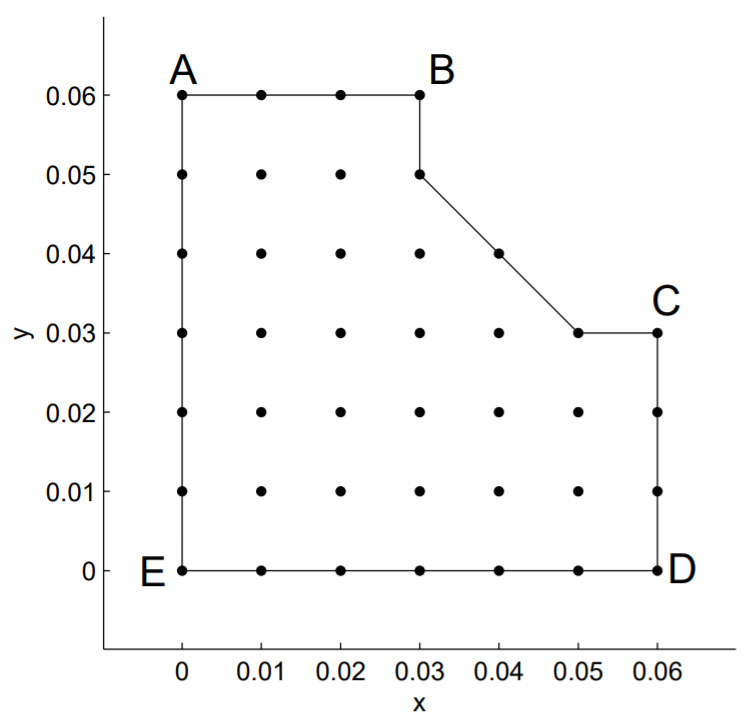
\includegraphics[width=\linewidth]{images/Component.png}
	\caption{Schematic of electronic component.}
	\label{fig:componentSchematic}
\end{figure}

The component schematic is shown in Figure \ref{fig:componentSchematic}. The location of the component within the device means it's subject to different temperature condition along it's boundaries. The boundary A-B is in perfect thermal contact with another component which the temperature is known to 70\degree C. The boundary C-D is also in perfect thermal contact with another component which the temperature is known to be 40\degree C. The boundary A-E-D is thermally insulated and the boundary B-C is exposed to the air at ambient temperature.

\subsection{Research methods}


\subsection{Limitations and assumptions}

\section{Discussion}

\subsection{Method}

\subsubsection{Procedures}

\subsubsection{Sample Size}

\subsubsection{Selection Criteria}

\subsection{Discussion and analysis of data}

\subsubsection{Issue 1}

\subsubsection{Issue 2}

\subsubsection{Issue 3}

\subsubsection{Reliability and accuracy of data}

\section{Conclusions}

\section{Recommendations}

\subsection{Recommendation 1}

\subsection{Recommendation 2}

\section{References}

\section{Appendices}

\section{Group Meeting Summaries}

\section{Statement of Contribution}
 
\end{document}